\documentclass[a4paper,11pt]{article}
\usepackage{amsmath}
\usepackage[english]{babel}
\usepackage{color}
\usepackage{graphicx}
\usepackage{hyperref}
\usepackage{subcaption}
\usepackage{mathabx}

\DeclareMathOperator*{\argmax}{arg\,max}
\DeclareMathOperator*{\Bern}{Bern}
\newcommand{\V}[1]{\ensuremath{\mathbf{#1}}}
\newcommand{\T}[1]{\ensuremath{\mathtt{#1}}}
\newcommand{\cA}{\ensuremath{C_\mathtt{A}}}
\newcommand{\cB}{\ensuremath{C_\mathtt{B}}}
\newcommand{\ck}{\ensuremath{C_k}}
\newcommand{\cML}{\ensuremath{C_{ML}}}
\newcommand{\muA}{\ensuremath{\boldsymbol{\mu}_\mathtt{A}}}
\newcommand{\muB}{\ensuremath{\boldsymbol{\mu}_\mathtt{B}}}
\newcommand{\muk}{\ensuremath{\boldsymbol{\mu}_k}}
\newcommand{\mean}{\ensuremath{\boldsymbol{\mu}}}
\newcommand{\cov}{\ensuremath{\boldsymbol{\Sigma}}}
\newcommand{\covA}{\ensuremath{\boldsymbol{\Sigma}_\mathtt{A}}}
\newcommand{\covB}{\ensuremath{\boldsymbol{\Sigma}_\mathtt{B}}}
\newcommand{\covk}{\ensuremath{\boldsymbol{\Sigma}_k}}
\newcommand{\mcA}{\ensuremath{\pi_\mathtt{A}}}
\newcommand{\mcB}{\ensuremath{\pi_\mathtt{B}}}
\newcommand{\mck}{\ensuremath{\pi_{k}}}
\newcommand{\mc}{\ensuremath{\boldsymbol{\pi}}}

\newcommand{\hl}[1]{\colorbox{cyan}{#1}}
\newcommand{\mhl}[1]{\mathchoice%
  {\colorbox{cyan}{$\displaystyle#1$}}%
  {\colorbox{cyan}{$\textstyle#1$}}%
  {\colorbox{cyan}{$\scriptstyle#1$}}%
  {\colorbox{cyan}{$\scriptscriptstyle#1$}}}

\title{Lab 3: Expectation Maximisation}
\author{Patrick de Kok}
\begin{document}
\maketitle

In this lab assignment, the datasets of both \texttt{banana.mat} and \texttt{spiral.mat} have been analyzed. 

\section{Gaussian Distribution}
\begin{figure}
\begin{center}
\caption{A plot of the dataset \texttt{banana.mat}.  The red ``$\color{red}+$'''s and magenta ``$\color{magenta}\mbox{o}$'''s represent the train and test data points from class A.  The blue ``$\color{blue}\times$'''s and cyan ``$\color{cyan}\convolution$'''s represent the train and test data points from class B.}
\label{fig:banana}
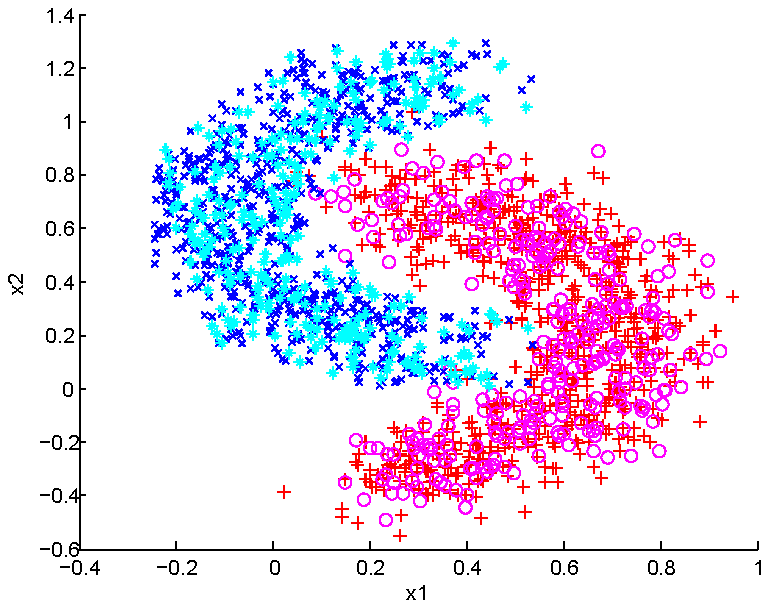
\includegraphics[width=\textwidth]{banana}
\end{center}
\end{figure}

\begin{figure}
\begin{center}
\caption{A plot of the dataset \texttt{spiral.mat}.  The red ``$\color{red}+$'''s and magenta ``$\color{magenta}\mbox{o}$'''s represent the train and test data points from class A.  The blue ``$\color{blue}\times$'''s and cyan ``$\color{cyan}\convolution$'''s represent the train and test data points from class B.}
\label{fig:spiral}
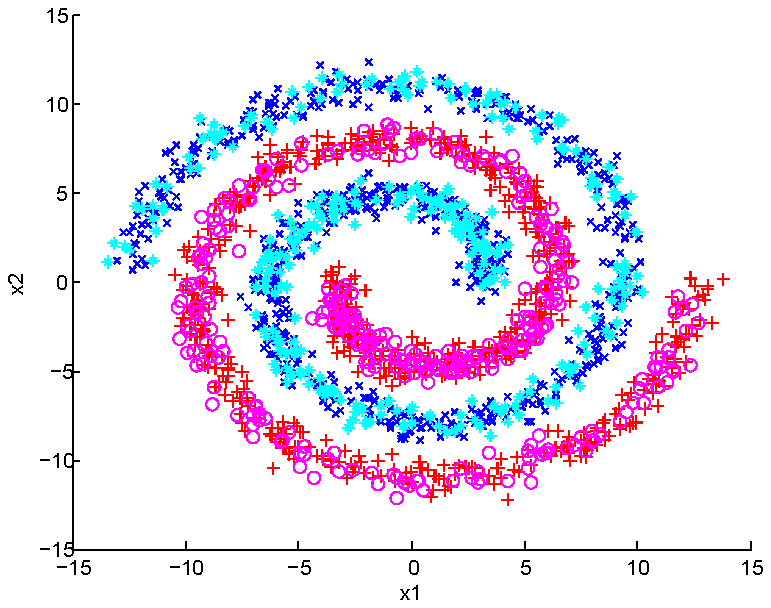
\includegraphics[width=0.8\textwidth]{spiral}
\end{center}
\end{figure}

In this exercise, I have trained a classifier, based on a single Gaussian distribution for each class of both datasets.

For \hl{testing}, I use the last $\mhl{30 \%}$ of both datasets.  Both datasets have \hl{not been shuffled}.  The train and test sets of \texttt{banana.mat} and \texttt{spiral.mat} have been plotted in \hl{\autoref{fig:banana} and \autoref{fig:spiral}}.

The training of the classifiers has been done as follows.  For both classes $\cA$ and $\cB$, the mean $\mean = [\muA, \muB]$ and covariances $\cov = [\covA, \covB]$ are computed.  For this assignment, I have assumed that the frequencies of $\cA$ and $\cB$ are representative of the real distribution.  Therefore, $\mhl{p(\ck)}$ is equal to \hl{the number of data points of class $\ck$, divided by the total number of data points}.  I then compute the most likely class \cML(\V{y}) for a data point $\V{y}$:
\begin{align*}
\cML(\V{x}) &= \argmax_{\ck} p(\V{x} | \ck) \\
    &= \argmax_{\ck} \frac{p(\ck | \V{x}) p(\ck)}{\sum_j p(\V{x} | C_j) p(C_j)} \\
    &= \argmax_{\ck} p(\ck | \V{x}) p(\ck) \\
    &= \argmax_{\ck} \mathcal{N}(\V{x} ; \muk, \covk) p(\ck)
\end{align*}

In MATLAB, the probability density function $\mathcal{N}(\V{x} ; \mean, \cov)$ is computed by \texttt{mvnpdf(x, MU, SIGMA)}.

This computation for \hl{\texttt{banana.mat} results in the confusion matrix and error rate}:
\begin{align*}
CM(\cML, \mbox{\texttt{banana.mat}}) 
    &= \left[ \begin{array}{cc}
      273 & 41 \\
      27 & 259\end{array}\right] \\
err(\cML, \mbox{\texttt{banana.mat}})
    &= 0.1133
\end{align*}

The corresponding values for \texttt{spiral.mat} are:
\begin{align*}
CM(\cML, \mbox{\texttt{spiral.mat}})
    &= \left[ \begin{array}{cc}
      219 & 110 \\
      81 & 190
\end{array}\right] \\
err(\cML, \mbox{\texttt{banana.mat}})
    &= 0.3183
\end{align*}


\section{Mixtures of Gaussians}
In the second exercise, a classifier will be trained to recognize the classes of the \texttt{banana.mat} and \texttt{spiral.mat} datasets, based on the EM algorithm.

% TODO section on EM?

The iterative loop of the EM algorithm has been implemented already, as well as a visualization module, which is called in every iteration.  To make everything work, I have implemented the following three MATLAB functions.
\begin{itemize}
\item \texttt{MOG = init\_mog(X, C)}.  Given the data and the desired number of Gaussians, compute the mean \texttt{MU}, covariance \texttt{SIGMA} and mixing coefficient \texttt{PI} for each Gaussian.  This is stored in \texttt{MOG}, a \texttt{C}-by-1 cell array of structures containing only these three keys.  For the $\T{k}$th element of \texttt{MOG}, \texttt{MU}, \texttt{SIGMA} and \texttt{PI} in the software correspond with the mathematical concepts of $\muk$, $\covk$ and $\mck$.  Another possible initialization is filling $\muk$, $\covk$ and $\mck$ with random values within the range of the dataset, for all possible values of $k$.  I have not tried doing so, as I expect this to be less effective.
%
\item \texttt{[Q LL] = mog\_E\_step(X, MOG)}.  This implements the expectation step of the EM algorithm.  For each data point $\mathtt{x} = \mathtt{X(n, :)}$ and the $\T{k}$th mixture with mean $\muk$, covariance $\covk$ and mixing coefficient $\mck$, the responsibility $\mck \mathcal{N}(\T{x} ; \muk, \covk)$ is divided by the sum of all responsibilities of the $\T{k}$th mixture, and stored in $\T{Q(n, k)}$, a $\T{N}$-by-$\T{C}$ matrix.  This corresponds with equation 9.13 of \cite{Bishop}:
\begin{align*}
\T{Q(n, k)} = \gamma(z_k) \equiv p(z_k = 1 | \V{x}) 
    &= \frac{p(z_k = 1) p(\V{x} | z_k = 1)}{\sum_{j=1}^{k} p(z_j = 1) p(\V{x} | z_j = 1)} \\
    &= \frac{\mck \mathcal{N}(\V{x} ; \muk, \covk)}{\sum_{j=1}^{k} \pi_j \mathcal{N}(\V{x} ; \muk, \covk)}
\end{align*}
However, in my implementation, only one iterator is used; MATLAB can compute the Gaussian distribution for a \texttt{N}-by-\texttt{D} matrix, given a 1-by-\texttt{D} mean and \texttt{D}-by-\texttt{D} covariance matrix.  Another speedup is computing the denominator \texttt{d} together with the numerator, and only dividing each \texttt{Q(n, k)} when the complete denominator is known.

$\T{LL}$ is the log-likelihood of the dataset under the mixture model.  This is computed corresponding to equation 9.14 of \cite{Bishop}:
\begin{align*}
\T{LL} = \ln p(\V{X} | \mc, \mean, \cov) &= \sum_{n=1}^{N} \ln \left\{ \sum_{k=1}^{C} \mck \mathcal{N}(\V{x}_n ; \muk, \covk) \right\}
\end{align*}
Because the innermost sum is the same as \texttt{d}, the implementation of this formula only takes marginally more time when \texttt{Q} is already computed.
%
\item \texttt{MOG = mog\_M\_step(X, Q, MOG)}.  This function updates the mean \texttt{MU}, covariance \texttt{SIGMA} and mixing coefficient \texttt{PI} in each cell of \texttt{MOG}.  For each \texttt{k}th element, this is done according to equations 9.17, 9.19 and 9.22 of \cite{Bishop}:
\begin{align*}
\muk &= \frac{1}{N_k} \sum_{n=1}^{N} \gamma(z_{nk}) \V{x}_n \\
\covk &= \frac{1}{N_k} \sum_{n=1}^{N} \gamma(z_{nk}) (\V{x}_n - \muk) (\V{x}_n - \muk)^T \\
\mck &= \frac{N_k}{N}
\end{align*}
where $N$ is the number of data points in \texttt{X}, $\V{x}_n$ corresponds with the $n$th row of \texttt{X} and $N_k$ is defined by equation 9.18:
\begin{align*}
N_k = \sum_{n=1}^{N} \gamma(z_{nk})
\end{align*}
such that $N = \sum_{k=1}^{\T{C}} N_k$.

There are some things that do not follow straightforward from these definitions to the implementation.  

Note that $\T{Q(n,k)}$ corresponds with $\gamma(z_{nk})$. $N_k$ is implemented as a 1-by-\texttt{C} row vector, generated by summing over all rows of \texttt{Q}.

Because the mean and data points are stored as row vectors, the transpose operator is placed on the first difference vector in the computation of $\covk$:
\begin{align*}
\covk &= \frac{1}{N_k} \sum_{n=1}^{N} \T{Q(n,k)} (\T{x}_n - \muk)^T (\T{x}_n - \muk)
\end{align*}

$\covk$ is only updated if it is non-singular.  In the code, this is defined as $\T{cond(}\covk\T{)} < 10^{10}$.  If $\covk$ is singular, the Gaussian has a really small area (almost no area) with high probabilities, so that almost no data point will be covered by it.

\end{itemize}

Finding the most likely class for the data is done in a similar fashion as for the previous exercise:

\begin{align*}
\cML(\V{x}) &= \argmax_{\ck} p(\V{x} | \ck) \\
    &= \argmax_{\ck} p(\ck) \sum_j p(\V{x}_n | z_j, \ck) p(z_j | \ck) \\
    &= \argmax_{\ck} p(\ck) \sum_j \mathcal{N}(\V{x}_n ; \mean_{jk}, \cov_{jk}) p(z_j | \ck)
    &= \argmax_{\ck} p(\ck) \sum_j \mathcal{N}(\V{x}_n ; \mean_{jk}, \cov_{jk}) \pi_{jk}
\end{align*}

I have tested the test data of both datasets for different models involving 1 through 40 Gaussian mixtures.  The error rate of the test set of the \texttt{banana.mat} dataset is plotted against the number of Gaussian mixtures in \autoref{fig:bananaerr}.  Similar data is plotted in \autoref{fig:spiralerr} for the \texttt{spiral.mat} data set.  

\begin{figure}
\begin{center}
\caption{The number of Gaussians plotted against the error rate for the \texttt{banana.mat} dataset.}
\label{fig:bananaerr}
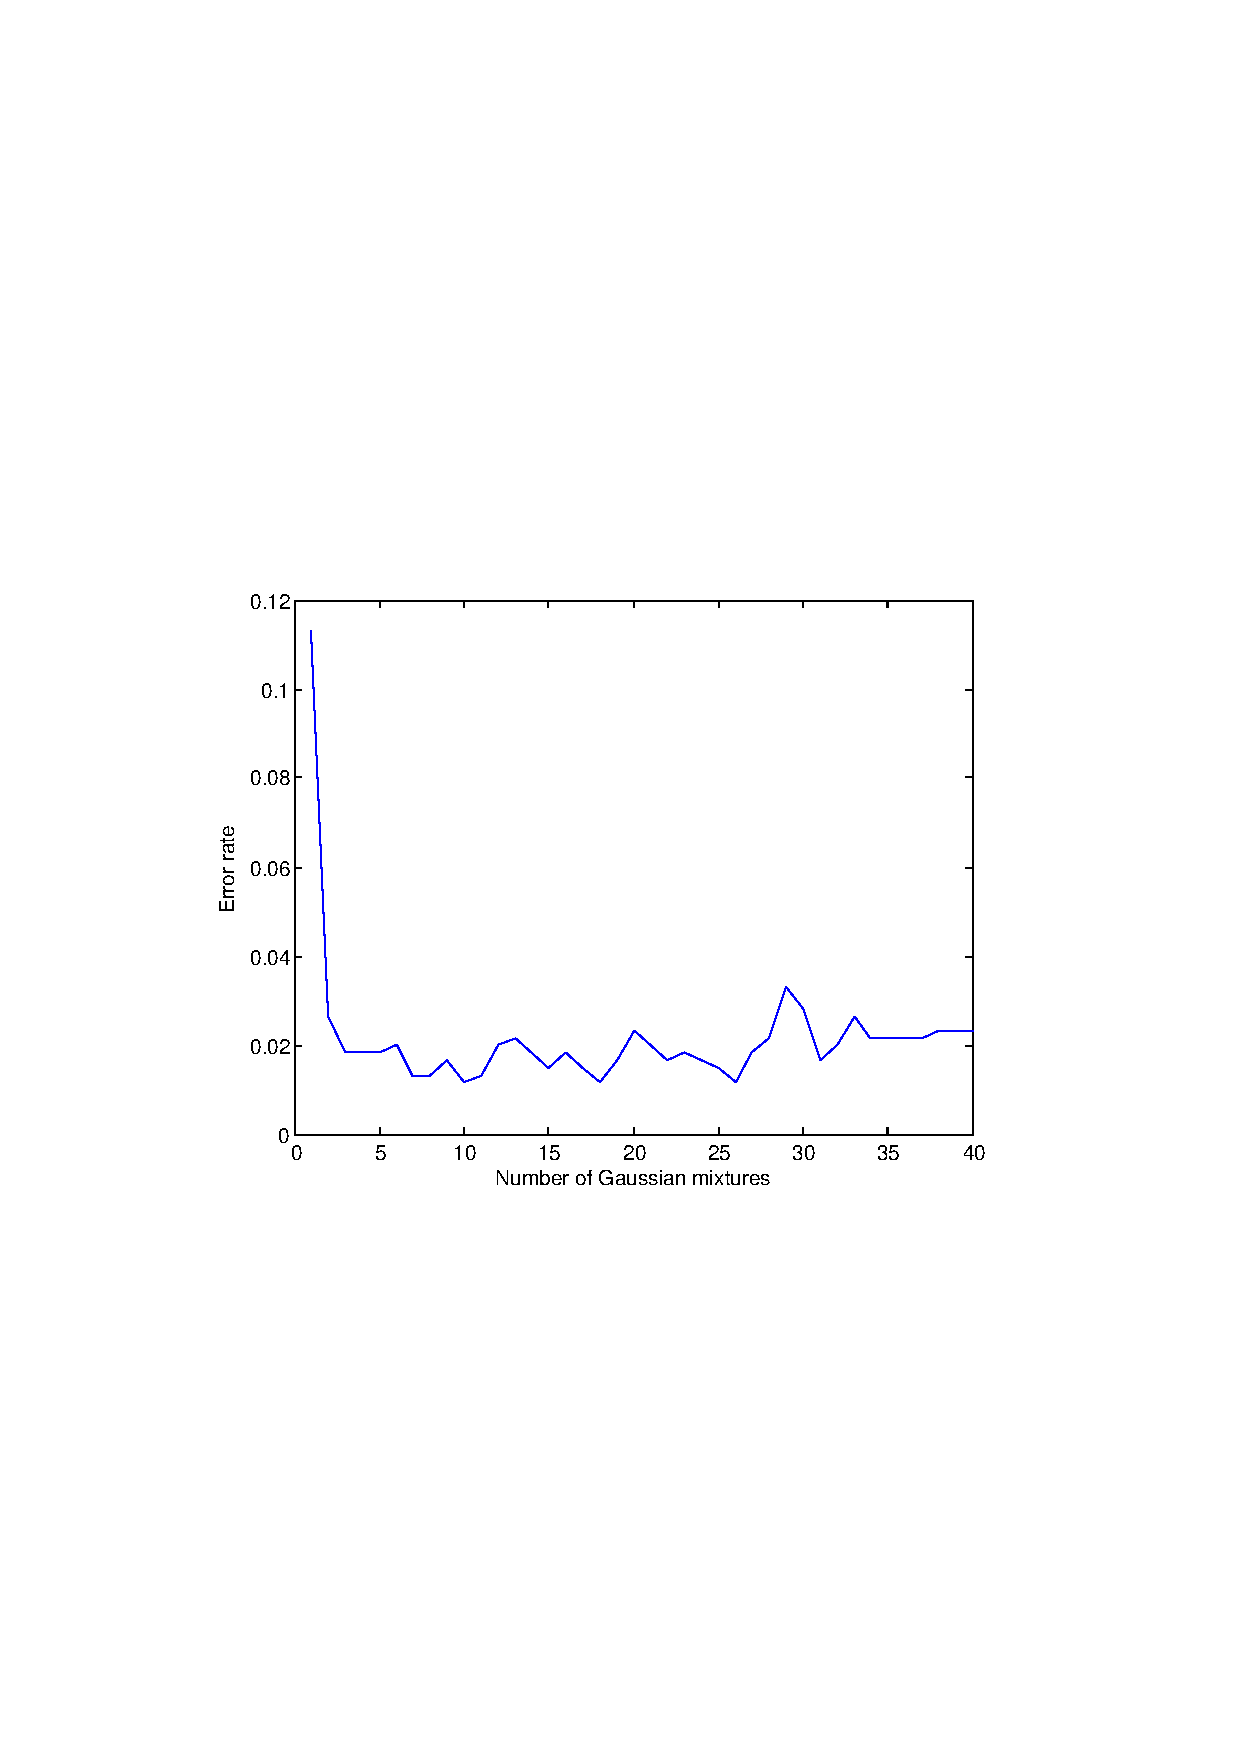
\includegraphics[width=\textwidth]{bananaerr}
\end{center}
\end{figure}

\begin{figure}
\begin{center}
\caption{The number of Gaussians plotted against the error rate for the \texttt{spiral.mat} dataset.}
\label{fig:spiralerr}
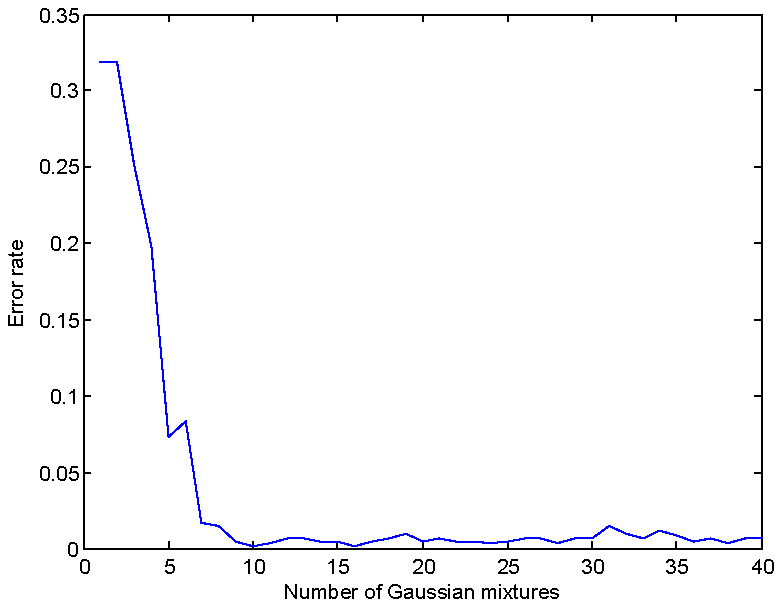
\includegraphics[width=\textwidth]{spiralerr}
\end{center}
\end{figure}

\begin{enumerate}
\item What is a sensible way to initialize the parameters of your model
\item How many components should you try?  Having plotted the data, can you guess what number of components should be optimal?  How does your classification accuracy evolve as the number of components change?
\item Do the results depend on the initialisation?
\item Why is hint 1 important?
\end{enumerate}

\section{Log-Probabilities}


\begin{enumerate}
\item
First implement a function called logsumexp that computes the sum of two log-probabilities as described above. Make sure that this function takes the largest value out of the logarithm. Write the function so that both scalars and matrices can be used as arguments

\item 
Discuss how we can use this function to compute sums of more than two probabilities using log-probabilities.

\item
Check your implementation by computing ln[p(a) + p(b)] when ln p(a) = −1000 and ln p(b) = −1001.

\item
Now convert the E-step of the previous exercise. Use the function lmvnpdf(X,MU,SIGMA) which is functionally equivalent to log mvnpdf(X,MU,SIGMA) but never computes the logarithm or exponent and is therefore numerically stable:

Notice, however, that only the function mog E step is changed, and that it must still return p(z|x, θ),
not ln p(z|x, θ). In the adapted function, you compute ln p(z|x, θ), but you need to exponentiate it before
returning the value. However now the computation does not suffer from the underflows and is therefore more
precise.
Include the pseudocode for logsumexp in your report, and write down what the E-step becomes when
using log-probabilities. Discuss how this affects your results.
\end{enumerate}


\bibliographystyle{alpha}
\bibliography{references}
\end{document}
